\chapter{Simulations} \label{chap-3}

One purpose of this chapter is to briefly describe the computational model used in the PyORBIT code before displaying any simulation results. The second purpose of this chapter is to review the work of Holmes et al., who performed particle-in-cell (PIC) simulations in the original ORBIT code to determine the feasibility of elliptical painting in the SNS \cite{Holmes2018}. 



\section{Computational model}

\subsection{Single-particle tracking}

PyORBIT tracks a Bunch object containing a set of 6D phase space coordinates. The accelerator is modeled as a series of nodes, each of which modifies the coordinates in some way. The core of PyORBIT is comprised of single-particle tracking routines. For dipoles, quadrupoles, and solenoids, full linear transport is used. The approach to handling nonlinear elements is inspired by TEAPOT (Thin-Element Accelerator Program for Optics and Tracking), where particles pass through a series of drifts and "kicks" from thin elements — elements with infinitesimal length \cite{Schachinger1987}. Each drift changes the particle's position without changing its momentum, while each kick changes the particle's momentum without changing its position. Thick elements are then approximated as a series of thin elements connected with drifts. The momentum kicks are derived from the Hamiltonian of a charged particle in an electromagnetic field. It can be shown that for a Hamiltonian $H$ that does not explicitly depend on $s$ (the time-like variable), then over a distance $L$, a function $g$ of the canonical coordinates will transform as
%
\begin{equation}
    g \rightarrow 
    = e^{-L:H:} g
    = \sum_{n=0}^{\infty}{\frac{L^n}{n!} (-:H:)^n g},
\end{equation}
%
where the operator $:H:$ is defined by
%
\begin{equation}
    \{H, g\} \equiv \, :H: g =
    \frac{\partial{H}}{\partial{\mathbf{q}}}
    \cdot
    \frac{\partial{g}}{\partial{\mathbf{p}}}
    -
    \frac{\partial{H}}{\partial{\mathbf{p}}}
    \cdot
    \frac{\partial{g}}{\partial{\mathbf{q}}}
\end{equation}
%
\cite{Dragt2018, Forest1998}. Symplectic maps connecting the initial and final phase space coordinates are then derived for various elements.

Fringe fields need to be taken into account for elements of finite length, that is, the fields outside the start and end of the element. For example, the magnetic field in a solenoid has a transverse component near the edges that vanishes in the limit of infinite length. The strength of fringe fields generally increases with the transverse distance from the center of the magnet; they are especially important in the injection region, where the closed orbit is significantly displaced from the quadrupole centers. PyORBIT handles fringe fields using a hard-edge model in which a nonlinear mapping is applied at the start and end of the magnet \cite{Forest1998}.

Longitudinal dynamics have not yet been discussed. Longitudinal focusing in the SNS ring is provided by four RF cavities. The harmonic number $h$, which is defined as the RF frequency divided by the revolution frequency of the beam, takes the value $h = 1$ in three cavities and $h = 2$ in one cavity. resulting in two peaks in the distribution. The cavities were designed to operate at 40 kV total for the first harmonic and 20 kV for the second harmonic, but after years of operational experience, they were lowered to their current values of approximately 5 kV. The energy gain for a particle passing through the cavity is approximated as $q V \sin(h \phi + \phi_0)$ where the particle phase $\phi$ is zero for the synchronous particle.\footnote{Since there is no net acceleration in the SNS ring, $\phi_0 = 0$.} Since particles see different accelerating voltages depending on their arrival time, they oscillate in a stable region of longitudinal phase space. The longitudinal tune is four orders of magnitude smaller than the transverse tune in the SNS ring.



\subsection{Collective effects}

The calculation of collective effects is a major component of high-intensity beam physics simulations. We focus first on space charge. PyORBIT uses the particle-in-cell (PIC) approach in which an $N$ particle bunch is represented by $M$ macroparticles, where $M \ll N$. The macroparticles are tracked according to the single-particle equation of motion (Eq.~\eqref{eq:eom_with_spacecharge}). The electric field is obtained by solving the Poisson equation (Eq.~\eqref{eq:Poisson}) on a grid. The key step is transforming between the discrete and continuous representations of the bunch.

The PIC loop is shown in Fig.~\ref{fig:pic_loop}. 
%
\begin{figure}[!p]
    \centering
    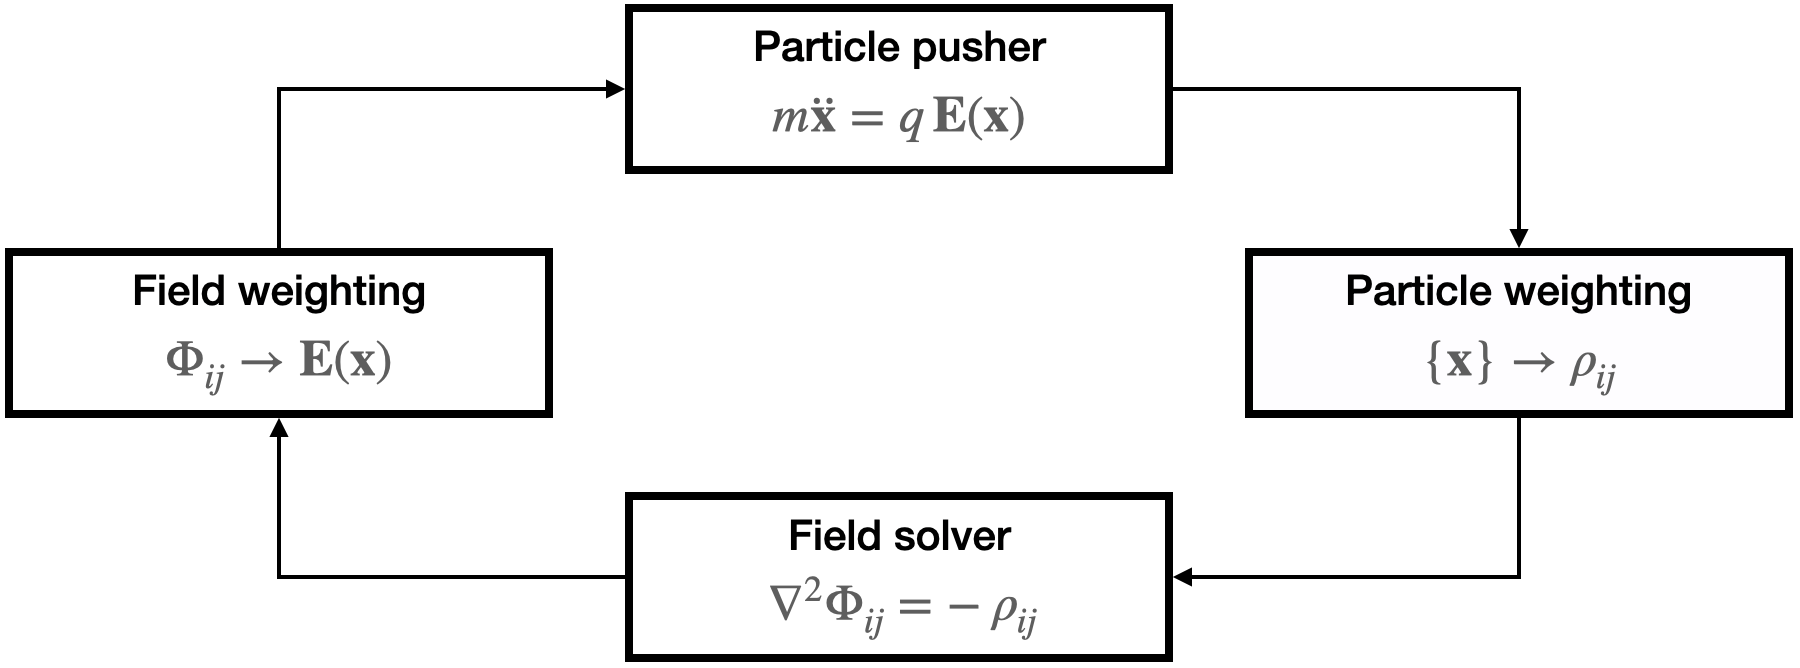
\includegraphics[width=\textwidth]{Images/chapter3/pic_loop.png}
    \caption{\label{fig:pic_loop}The particle-in-cell loop.}
\end{figure}
%
First, the charge density $\rho_{i,j}$ is obtained on a grid. A common method is to treat each macroparticle as a rectangular, uniform density cloud of charge with dimensions equal to the grid spacing, assigning a fractional charge to each bin according to the fraction of the cloud overlapping with that bin \cite{Birdsall1975}. Second, the Poisson equation is solved on the grid. The method used in PyORBIT follows \cite{Hockney1981}, where the potential is written as the convolution ($*$) of a Green's function\footnote{Here we take a stand on the ``Green's function" vs. ``Green function" debate \cite{Wright2006}.} $G(\mathbf{x})$ with the charge density $\rho(\mathbf{x})$:
%
\begin{equation}
    \Phi(\mathbf{x}) = G(\mathbf{x}) * \rho(\mathbf{x}).
\end{equation}
%
We then exploit the convolution theorem \cite{Arfken1985} to write the Fourier transform ($\mathcal{F}$) of the potential as the direct product of the Fourier transforms of the Green's function and charge density:
%
\begin{equation}
    \mathcal{F}[\Phi(\mathbf{x})]
    =
    \mathcal{F}[G(\mathbf{x})] \cdot \mathcal{F}[\rho(\mathbf{x})].
\end{equation}
%
For a grid with $N$ total points, the time-complexity of the convolution is $O(N^2)$. The Fourier transform reduces this to $O(N \log N)$. To create periodic boundary conditions, the grid is doubled in each dimension; in the new regions, the Green's function is mirror-reflected and the charge density is set to zero. The potential is then solved for on the doubled grid, after which only the original region is kept. An example is shown in Fig.~\ref{fig:poisson}. 
%
\begin{figure}[!p]
    \centering
    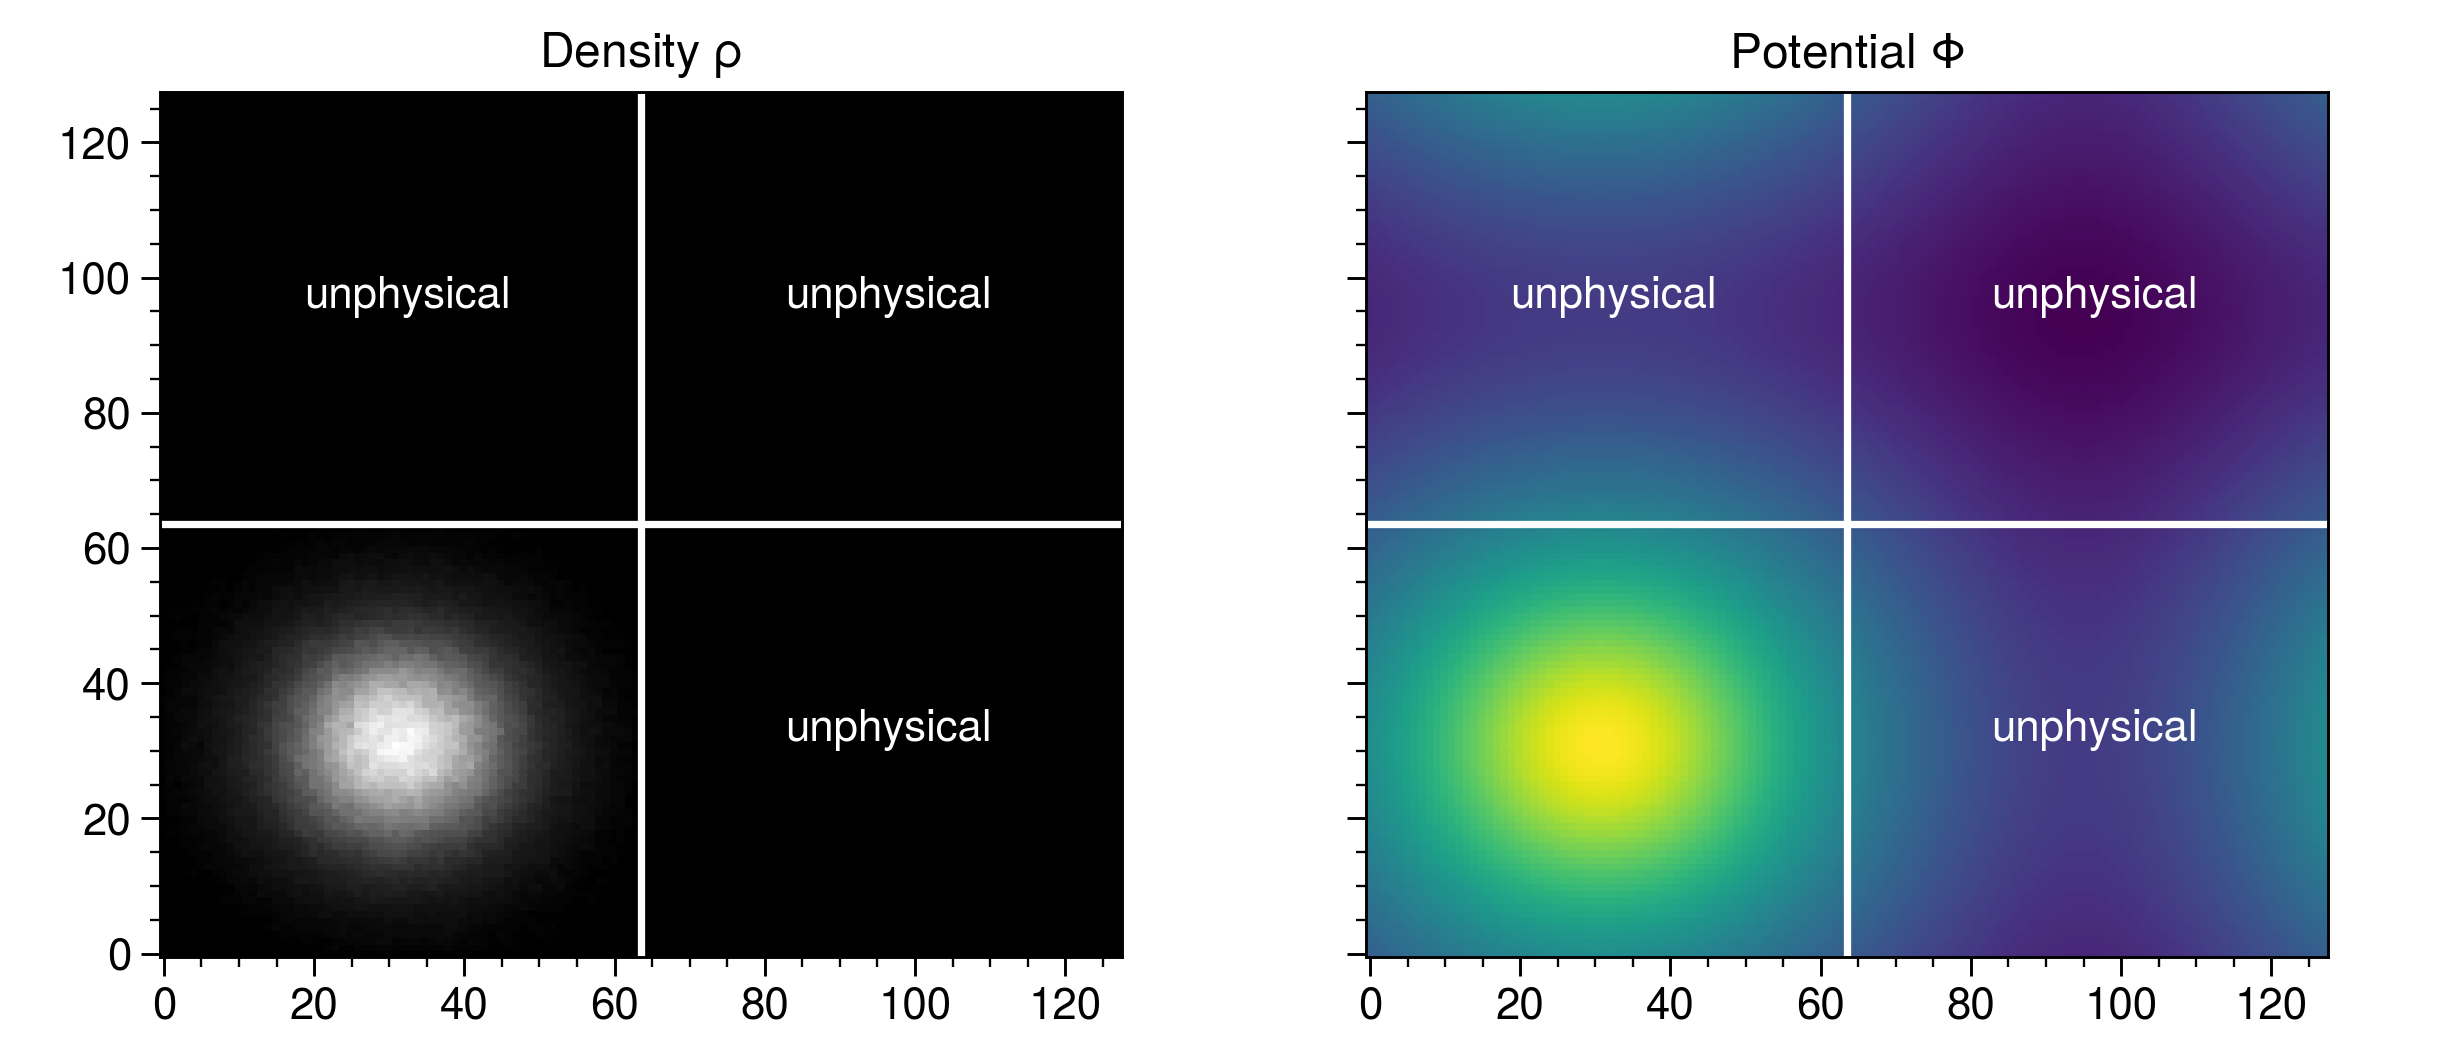
\includegraphics[width=\textwidth]{Images/chapter3/poisson.png}
    \caption{\label{fig:poisson}Solution of the Poisson equation on a doubled grid.}
\end{figure}
%
Third, using the same weighting method as the first step, the gradient of the potential is interpolated at the particle positions. Finally, the particle momenta are updated using an appropriate integration scheme.

In rings where the coasting beam approximation is valid, the longitudinal and transverse dimensions can be treated separately. In PyORBIT, a longitudinal space charge node, which solves the Poisson equation for the 1D projection of the distribution onto the $z$ axis, acts on the bunch once per turn. Transverse space charge nodes are distributed throughout the ring. The model used in this work is known as the sliced model: the bunch is sliced into longitudinal segments, and the Poisson equation is individually solved for each segment's projection onto the $x$-$y$ plane.

In the discussion of space charge thus far, the beam was assumed to be in free space; in reality, the beam is in a vacuum chamber such as a conducting pipe. This has two effects. First, the boundary conditions must be applied when solving the Poisson equation. Second, each charged particle interacts with the vacuum chamber, leaving a wake field that affects trailing particles or the same particle on subsequent turns, possibly leading to instability. The treatment of wake fields is introduced in \cite{Chao1993}. No details are described here; we only mention that PyORBIT takes these effects into account and has been benchmarked against experiments \cite{Holmes2011}.






\subsection{Simulation procedure}

PyORBIT employs a two-language scheme: the core algorithms are written in C++ but are accessed at the Python level. All PyORBIT scripts are written in Python. The scripts used in this work are modified versions of previously benchmarked injection scripts.

For space charge calculations, a 128 $\times$ 128 $\times$ 64 grid is used with the sliced model. No more than 1 meter is allowed between solver nodes. The final number of particles is generally $5 \times 10^{5}$. With these settings, a 1000-turn injection simulation takes several days to run on a 2014 MacBook Pro with a 2.5 GHz Intel Core i7 processor, 16 GB of memory, and the macOS Mojave operating system.\footnote{These simulation parameters are not hard-wired into PyORBIT.}

In all simulations, the turn-by-turn covariance matrix of the distribution at the injection point is saved to a file. If space permits, the turn-by-turn 6D phase space coordinates at the injection point are saved to a single file as an array of size $n T (T + 1) / 2 \times 6$, where $n$ is the number of macroparticles injected per turn and $T$ is the total number of turns. (The array is reshaped during analysis to obtain a $T$-element list of coordinate arrays.) Additionally, the distribution is periodically saved at the ring extraction point so that it can be transported to the target in a separate simulation.





\section{Painting simulations}

\subsection{Injection}

Injection is simulated by adding particles to the bunch at the foil location on each turn. Since each pulse is the sum of many minipulses from the linac, it is only necessary to use an approximate representation of the minipulse. The distribution used in this work resembles a truncated Gaussian in the transverse plane. The design RMS emittance is approximately 0.3 mm~mrad, but recent measurements indicate that the emittance may be closer to 0.5 mm~mrad. Additionally, although the Twiss parameters are usually assumed to be matched to the ring ($\beta_x \approx \beta_y \approx 10$ m, $\alpha_x \approx \alpha_y \approx 0$), the measurements indicated that the $\beta$ functions may be closer to 4 m/rad and the alpha functions may be closer to -0.5. We use values close to these measurements. In the longitudinal plane, the spatial distribution is uniform and the energy distribution is a Gaussian with a mean of 1 GeV and a standard deviation of less than 1 MeV.

An important effect during charge-exchange injection is the scattering and energy loss that occurs during passage through the stripper foil, which increases the effective emittance of the injected bunch. The relevant processes are multiple Coloumb scattering, ionization energy loss, and single scattering interactions such as Rutherford elastic scattering, nuclear elastic scattering, and nuclear inelastic absorption \cite{Chao2012, Cousineau2003}. These are implemented as Monte Carlo routines in a foil node that acts on the bunch once per turn.

Phase space painting can be simulated by adding an artificial time-dependent bump to the coordinates on each turn; however, it is more realistic to vary the strengths of the eight injection kickers in the model with the inclusion of element offsets from the closed orbit. The following procedure is used to set the coordinates at the injection point: Let $(x_o, x'_o, y_o, y'_o)$ be the desired coordinates. First, a particle is launched from the injection point with $x = x_o$, $x' = x'_o$, and $y = y' = 0$. The particle is tracked to the end of the injection region. An optimizer varies two kicker strengths to flatten the downstream orbit, i.e., obtain $x = x' = 0$ after tracking. Then, the particle is launched with $x = x_o$, $x' = -x'_o$ and tracked backwards to the start of the injection region. Two kickers are varied to flatten the upstream orbit, i.e., obtain $x = x' = 0$ at the start of the injection region. The process is repeated with the vertical orbit.


\subsection{Best-case scenario}

Holmes et al. performed realistic simulations of elliptical painting in the SNS using the original ORBIT code \cite{Holmes2018}. Their final simulation produced an approximate Danilov distribution. Only the final 1D projections of the distribution were displayed in the publication, and the intrinsic emittances were not calculated, so it is worth revisiting these results. Projections of the final distribution are shown in Fig.~\ref{fig:Holmes_corner_compare}.
%
\begin{figure}[!p]
    \centering
    \begin{subfigure}{0.8\textwidth}
        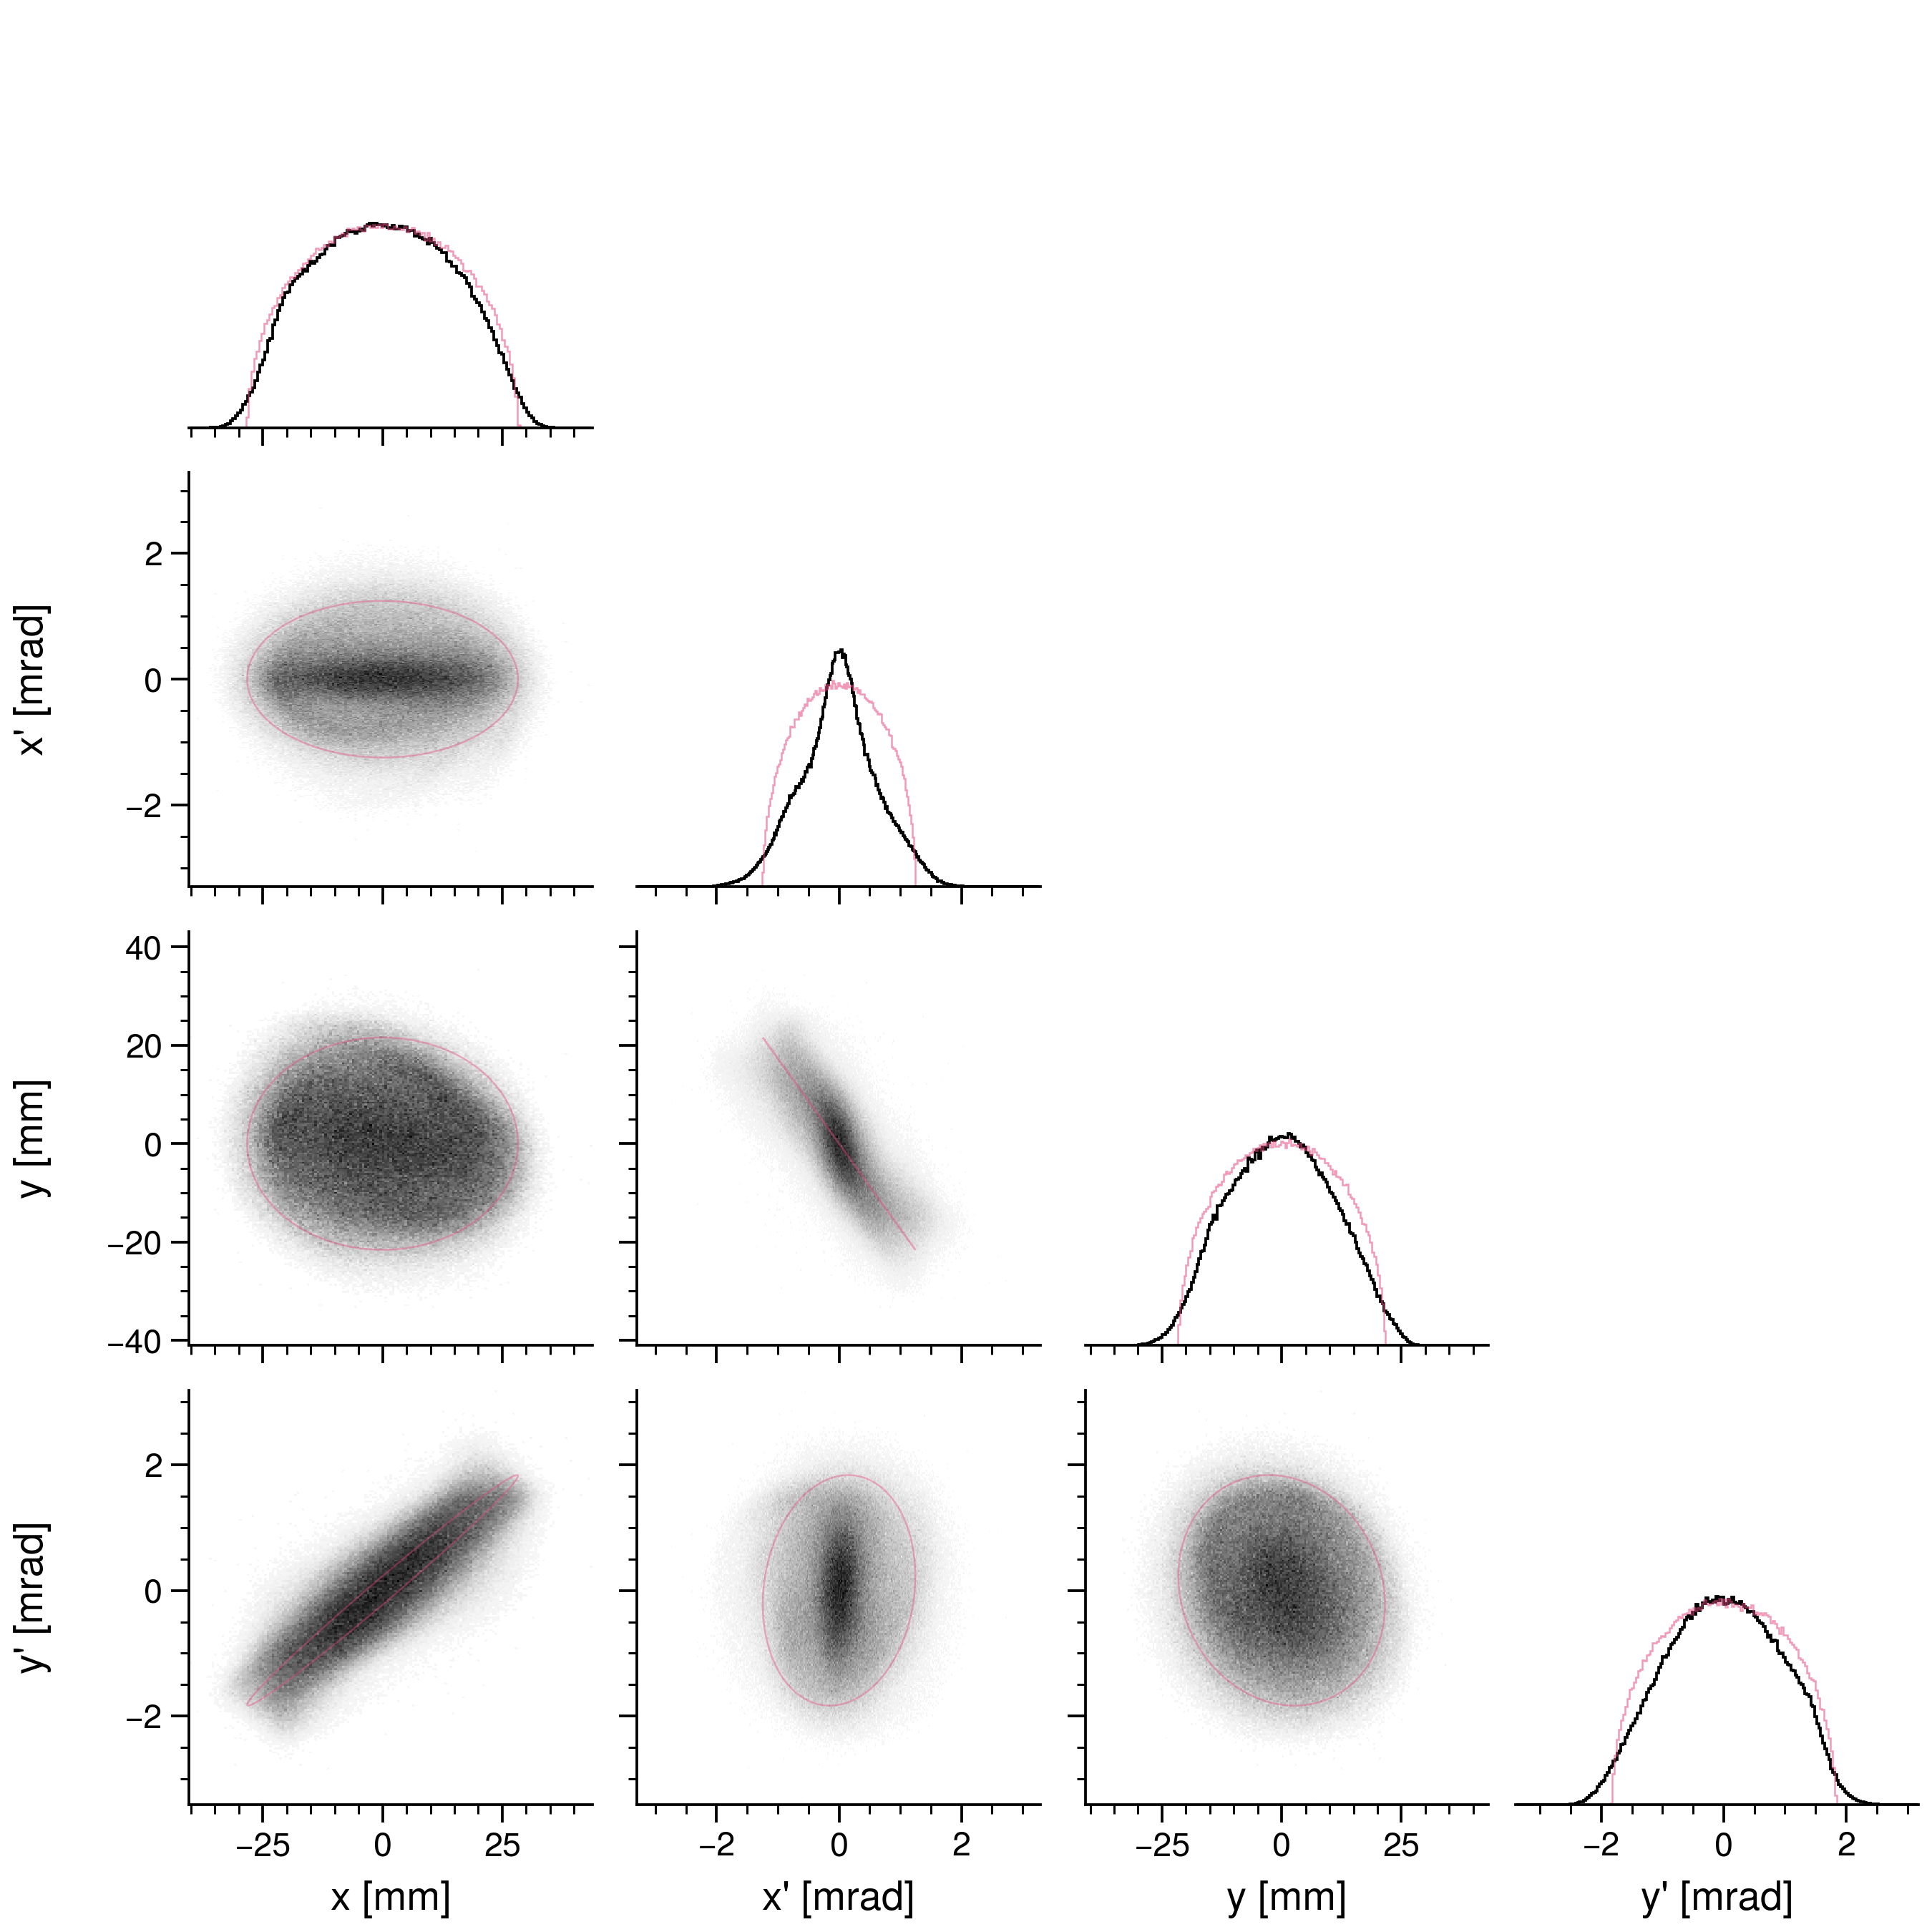
\includegraphics[width=\textwidth]{Images/chapter3/Holmes_corner_compare.png}
        \caption{1D and 2D projections of the final distribution at the injection point. The faint lines show the projections of an ideal Danilov distribution with the same Twiss parameters and apparent emittances as the simulated distribution.}
        \label{fig:Holmes_corner_compare}
    \end{subfigure}
    \vfill
    \vspace*{1.25cm}
    \vfill
    \begin{subfigure}{0.5\textwidth}
        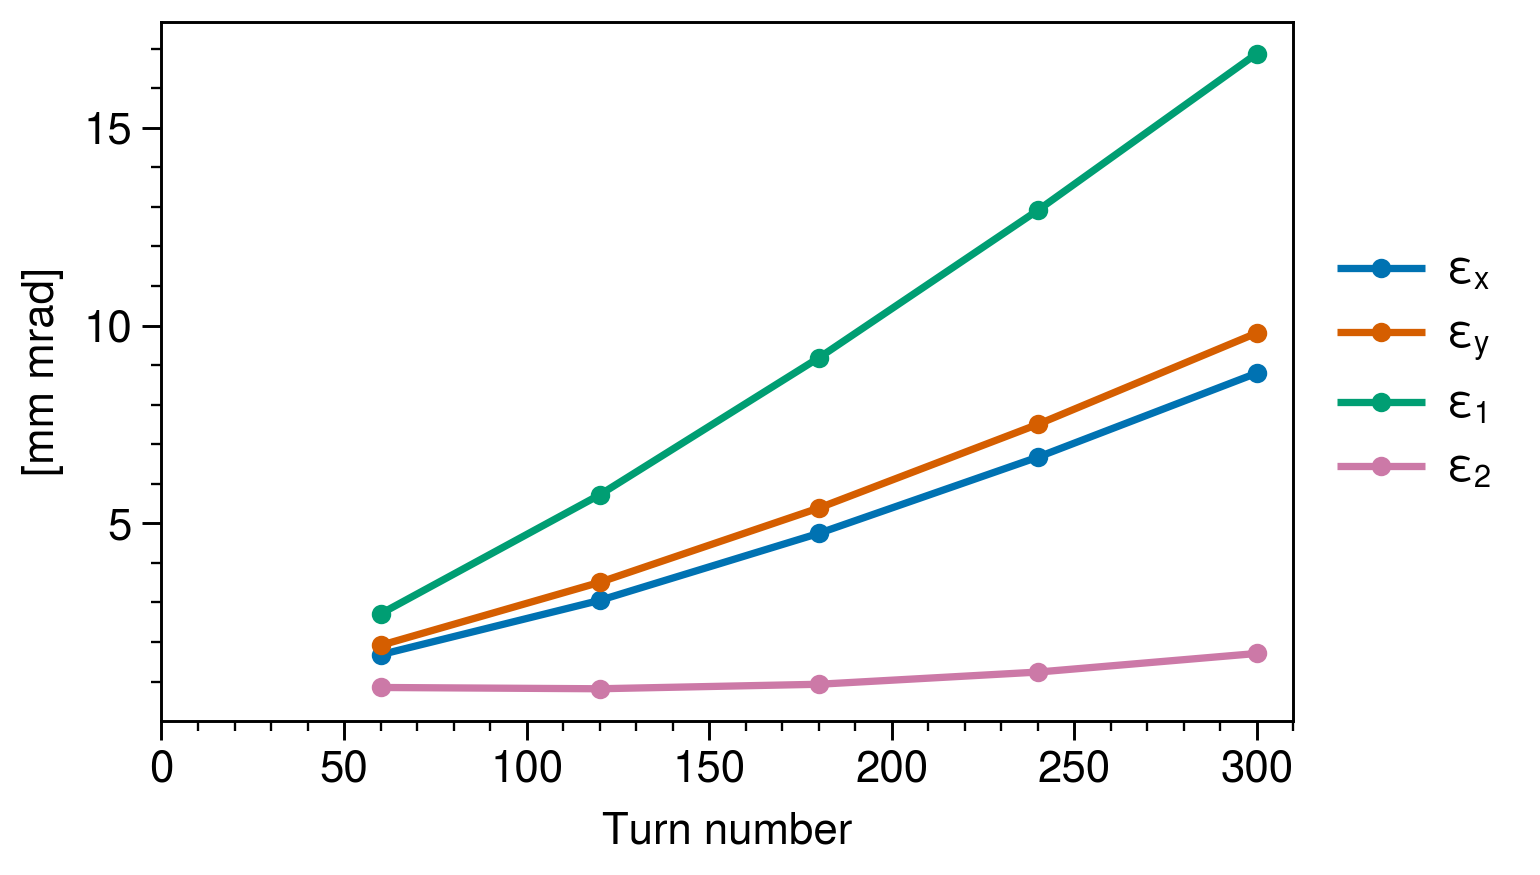
\includegraphics[width=\textwidth]{Images/chapter3/Holmes_emittances.png}
        \caption{RMS emittances every 60 turns during injection.}
        \label{fig:Holmes_emittances}
    \end{subfigure}
    \caption{Distribution from the final simulation in \cite{Holmes2018}.}
    \label{fig:Holmes}
\end{figure}
%
The faint pink lines represent the projections of an ideal Danilov distribution with the same Twiss parameters and apparent emittances as the simulated distribution. Although the 1D projections have developed tails, they are relatively close to the ideal case. The exception is the $x'$ projection, which has developed a sharp peak. The 2D projections are also not too far from ideal: the $x$-$y'$ and $y$-$x'$ projections have been broadened, but they exhibit the correct correlations, and the beam is round in the $x$-$y$ plane. Fig.~\ref{fig:Holmes_emittances} shows that the smaller intrinsic emittance remains close to its lower limit throughout injection, meaning that particles have been injected mostly into one mode. 

Several steps were necessary to achieve this simulated result. First, the painting path was chosen to follow a line in the $x$-$y'$ plane and the apparent emittances were kept somewhat equal; both these steps were discussed in Chapter \ref{chap-2}. Third, the ring RF cavity voltages were decreased to better approximate a coasting beam. Fourth, the beam energy was lowered to 0.6 GeV to increase the effective kicker strength; additionally, orbit corrector dipoles in the injection region provided a closed vertical bump. These modifications allowed a vertical slope of 1.58 mrad at the injection point. Fifth, the number of injected turns was reduced from 1000 to 300 to compensate for the increased space charge strength at the lower energy. Finally, a solenoid magnet was added to the ring to mitigate the effect of fringe fields. (The stabilizing effect of solenoids on the motion is examined in Appendix \ref{app-C}.)

It is encouraging that even with with inclusion of space charge, wake fields, nonlinear external fields, beam bunching, foil scattering, chromaticity, etc. simulations predict that an approximate Danilov distribution can be produced. This is likely the best-case-scenario in the SNS. But as will be discussed in Chapter \ref{chap-5}, new experimental constraints have come to light. The SNS cannot easily reach 0.6 GeV, and the use of orbit correctors in the injection region is difficult. The net result is that the maximum vertical injection angle may be limited (at least in initial experiments). Additionally, the minipulse may be mismatched at the injection point, but we expect this to have only a small effect if a sizeable beam is painted. Finally, solenoid magnets will not be installed in the SNS ring until a later date, so initial experiments will create elliptical modes in the ring by setting equal horizontal and vertical tunes. The distribution is expected to be less stable with such a machine configuration.\footnote{Holmes found that the beam should be somewhat insensitive to the tune split in the ring, but as mentioned in Chapter \ref{chap-3}, his studies were performed with a solenoid to the ring — the tune split was calculated without the solenoid.} Simulations with these constraints will be shown after several of the experiments in Chapter \ref{chap-5}.